\documentclass[twoside]{book}

% Packages required by doxygen
\usepackage{fixltx2e}
\usepackage{calc}
\usepackage{doxygen}
\usepackage[export]{adjustbox} % also loads graphicx
\usepackage{graphicx}
\usepackage[utf8]{inputenc}
\usepackage{makeidx}
\usepackage{multicol}
\usepackage{multirow}
\PassOptionsToPackage{warn}{textcomp}
\usepackage{textcomp}
\usepackage[nointegrals]{wasysym}
\usepackage[table]{xcolor}

% NLS support packages
\usepackage{hfont}

% Font selection
\usepackage[T1]{fontenc}
\usepackage[scaled=.90]{helvet}
\usepackage{courier}
\usepackage{amssymb}
\usepackage{sectsty}
\renewcommand{\familydefault}{\sfdefault}
\allsectionsfont{%
  \fontseries{bc}\selectfont%
  \color{darkgray}%
}
\renewcommand{\DoxyLabelFont}{%
  \fontseries{bc}\selectfont%
  \color{darkgray}%
}
\newcommand{\+}{\discretionary{\mbox{\scriptsize$\hookleftarrow$}}{}{}}

% Page & text layout
\usepackage{geometry}
\geometry{%
  a4paper,%
  top=2.5cm,%
  bottom=2.5cm,%
  left=2.5cm,%
  right=2.5cm%
}
\tolerance=750
\hfuzz=15pt
\hbadness=750
\setlength{\emergencystretch}{15pt}
\setlength{\parindent}{0cm}
\setlength{\parskip}{0.2cm}
\makeatletter
\renewcommand{\paragraph}{%
  \@startsection{paragraph}{4}{0ex}{-1.0ex}{1.0ex}{%
    \normalfont\normalsize\bfseries\SS@parafont%
  }%
}
\renewcommand{\subparagraph}{%
  \@startsection{subparagraph}{5}{0ex}{-1.0ex}{1.0ex}{%
    \normalfont\normalsize\bfseries\SS@subparafont%
  }%
}
\makeatother

% Headers & footers
\usepackage{fancyhdr}
\pagestyle{fancyplain}
\fancyhead[LE]{\fancyplain{}{\bfseries\thepage}}
\fancyhead[CE]{\fancyplain{}{}}
\fancyhead[RE]{\fancyplain{}{\bfseries\leftmark}}
\fancyhead[LO]{\fancyplain{}{\bfseries\rightmark}}
\fancyhead[CO]{\fancyplain{}{}}
\fancyhead[RO]{\fancyplain{}{\bfseries\thepage}}
\fancyfoot[LE]{\fancyplain{}{}}
\fancyfoot[CE]{\fancyplain{}{}}
\fancyfoot[RE]{\fancyplain{}{\bfseries\scriptsize 생성시간 \+: 월 3월 23 2015 22\+:47\+:09, 프로젝트명 \+: Home\+Flow, 생성자 \+:  Doxygen }}
\fancyfoot[LO]{\fancyplain{}{\bfseries\scriptsize 생성시간 \+: 월 3월 23 2015 22\+:47\+:09, 프로젝트명 \+: Home\+Flow, 생성자 \+:  Doxygen }}
\fancyfoot[CO]{\fancyplain{}{}}
\fancyfoot[RO]{\fancyplain{}{}}
\renewcommand{\footrulewidth}{0.4pt}
\renewcommand{\chaptermark}[1]{%
  \markboth{#1}{}%
}
\renewcommand{\sectionmark}[1]{%
  \markright{\thesection\ #1}%
}

% Indices & bibliography
\usepackage{natbib}
\usepackage[titles]{tocloft}
\setcounter{tocdepth}{3}
\setcounter{secnumdepth}{5}
\makeindex

% Hyperlinks (required, but should be loaded last)
\usepackage{ifpdf}
\ifpdf
  \usepackage[pdftex,pagebackref=true]{hyperref}
\else
  \usepackage[ps2pdf,pagebackref=true]{hyperref}
\fi
\hypersetup{%
  colorlinks=true,%
  linkcolor=blue,%
  citecolor=blue,%
  unicode%
}

% Custom commands
\newcommand{\clearemptydoublepage}{%
  \newpage{\pagestyle{empty}\cleardoublepage}%
}


%===== C O N T E N T S =====

\begin{document}

% Titlepage & ToC
\hypersetup{pageanchor=false,
             bookmarks=true,
             bookmarksnumbered=true,
             pdfencoding=unicode
            }
\pagenumbering{roman}
\begin{titlepage}
\vspace*{7cm}
\begin{center}%
{\Large Home\+Flow \\[1ex]\large 1.\+0.\+2 }\\
\vspace*{1cm}
{\large 다음에 의해 생성됨 \+:  Doxygen 1.8.9.1}\\
\vspace*{0.5cm}
{\small 월 3월 23 2015 22:47:09}\\
\end{center}
\end{titlepage}
\clearemptydoublepage
\tableofcontents
\clearemptydoublepage
\pagenumbering{arabic}
\hypersetup{pageanchor=true}

%--- Begin generated contents ---
\chapter{Home\+Flow android app}
\label{index}\hypertarget{index}{}\hypertarget{index_Author}{}\section{Author}\label{index_Author}

\begin{DoxyItemize}
\item Jongho L\+Im
\item Jinsung Choi 
\end{DoxyItemize}
\chapter{할일 목록}
\label{todo}
\hypertarget{todo}{}

\begin{DoxyRefList}
\item[\label{todo__todo000001}%
\hypertarget{todo__todo000001}{}%
클래스 \hyperlink{classkookmin_1_1cs_1_1homeflow_1_1_dashboard_activity}{kookmin.cs.homeflow.Dashboard\+Activity} ]Read workflow file(xml parse), check progress of workflow, etc...  
\item[\label{todo__todo000002}%
\hypertarget{todo__todo000002}{}%
클래스 \hyperlink{classkookmin_1_1cs_1_1homeflow_1_1_device_list_activity}{kookmin.cs.homeflow.Device\+List\+Activity} ]develop ...  
\item[\label{todo__todo000003}%
\hypertarget{todo__todo000003}{}%
클래스 \hyperlink{classkookmin_1_1cs_1_1homeflow_1_1_flow_list_activity}{kookmin.cs.homeflow.Flow\+List\+Activity} ]develop U\+I, List Item Click, Button Click etc...  
\item[\label{todo__todo000004}%
\hypertarget{todo__todo000004}{}%
멤버 \hyperlink{classkookmin_1_1cs_1_1homeflow_1_1_flow_list_activity_a8e7f4c315f0498cbb846022ddd0df21e}{kookmin.cs.homeflow.Flow\+List\+Activity.on\+Create} (Bundle saved\+Instance\+State)]read list of workflow xml file and show  
\item[\label{todo__todo000005}%
\hypertarget{todo__todo000005}{}%
클래스 \hyperlink{classkookmin_1_1cs_1_1homeflow_1_1_login_activity}{kookmin.cs.homeflow.Login\+Activity} ]function develop user check with server communication  
\item[\label{todo__todo000006}%
\hypertarget{todo__todo000006}{}%
멤버 \hyperlink{classkookmin_1_1cs_1_1homeflow_1_1_login_activity_a29cfa7fedc97be0ec337678df698100f}{kookmin.cs.homeflow.Login\+Activity.on\+Click} (View v)]implement function user check with server communication 
\end{DoxyRefList}
\chapter{네임스페이스 색인}
\section{패키지}
다음은 패키지들입니다. (가능한한 간략한 설명만을 보여줍니다) \+:\begin{DoxyCompactList}
\item\contentsline{section}{\hyperlink{namespacekookmin_1_1cs_1_1homeflow}{kookmin.\+cs.\+homeflow} \\*Java package of Home\+Flow app }{\pageref{namespacekookmin_1_1cs_1_1homeflow}}{}
\item\contentsline{section}{\hyperlink{namespacekookmin_1_1cs_1_1homeflow_1_1data}{kookmin.\+cs.\+homeflow.\+data} \\*Data classes of Home\+Flow app }{\pageref{namespacekookmin_1_1cs_1_1homeflow_1_1data}}{}
\end{DoxyCompactList}

\chapter{계통도 색인}
\section{클래스 계통도}
이 상속 목록은 완전하진 않지만 알파벳순으로 대략적으로 정렬되어있습니다.\+:\begin{DoxyCompactList}
\item \contentsline{section}{kookmin.\+cs.\+homeflow.\+data.\+Device}{\pageref{classkookmin_1_1cs_1_1homeflow_1_1data_1_1_device}}{}
\item \contentsline{section}{kookmin.\+cs.\+homeflow.\+data.\+Device.\+Function}{\pageref{classkookmin_1_1cs_1_1homeflow_1_1data_1_1_device_1_1_function}}{}
\item On\+Click\+Listener\begin{DoxyCompactList}
\item \contentsline{section}{kookmin.\+cs.\+homeflow.\+Login\+Activity}{\pageref{classkookmin_1_1cs_1_1homeflow_1_1_login_activity}}{}
\end{DoxyCompactList}
\item \contentsline{section}{kookmin.\+cs.\+homeflow.\+data.\+Workflow.\+Work}{\pageref{classkookmin_1_1cs_1_1homeflow_1_1data_1_1_workflow_1_1_work}}{}
\item \contentsline{section}{kookmin.\+cs.\+homeflow.\+data.\+Workflow}{\pageref{classkookmin_1_1cs_1_1homeflow_1_1data_1_1_workflow}}{}
\item Action\+Bar\+Activity\begin{DoxyCompactList}
\item \contentsline{section}{kookmin.\+cs.\+homeflow.\+Dashboard\+Activity}{\pageref{classkookmin_1_1cs_1_1homeflow_1_1_dashboard_activity}}{}
\item \contentsline{section}{kookmin.\+cs.\+homeflow.\+Device\+List\+Activity}{\pageref{classkookmin_1_1cs_1_1homeflow_1_1_device_list_activity}}{}
\item \contentsline{section}{kookmin.\+cs.\+homeflow.\+Flow\+List\+Activity}{\pageref{classkookmin_1_1cs_1_1homeflow_1_1_flow_list_activity}}{}
\item \contentsline{section}{kookmin.\+cs.\+homeflow.\+Login\+Activity}{\pageref{classkookmin_1_1cs_1_1homeflow_1_1_login_activity}}{}
\end{DoxyCompactList}
\item Application\+Test\+Case\begin{DoxyCompactList}
\item \contentsline{section}{kookmin.\+cs.\+homeflow.\+Application\+Test}{\pageref{classkookmin_1_1cs_1_1homeflow_1_1_application_test}}{}
\end{DoxyCompactList}
\end{DoxyCompactList}

\chapter{클래스 색인}
\section{클래스 목록}
다음은 클래스, 구조체, 공용체 그리고 인터페이스들입니다. (간략한 설명만을 보여줍니다) \+:\begin{DoxyCompactList}
\item\contentsline{section}{\hyperlink{classkookmin_1_1cs_1_1homeflow_1_1_application_test}{kookmin.\+cs.\+homeflow.\+Application\+Test} }{\pageref{classkookmin_1_1cs_1_1homeflow_1_1_application_test}}{}
\item\contentsline{section}{\hyperlink{classkookmin_1_1cs_1_1homeflow_1_1_dashboard_activity}{kookmin.\+cs.\+homeflow.\+Dashboard\+Activity} \\*Activity is dashboard of the progress of workflow }{\pageref{classkookmin_1_1cs_1_1homeflow_1_1_dashboard_activity}}{}
\item\contentsline{section}{\hyperlink{classkookmin_1_1cs_1_1homeflow_1_1data_1_1_device}{kookmin.\+cs.\+homeflow.\+data.\+Device} \\*Class is data of \hyperlink{classkookmin_1_1cs_1_1homeflow_1_1data_1_1_device}{Device} }{\pageref{classkookmin_1_1cs_1_1homeflow_1_1data_1_1_device}}{}
\item\contentsline{section}{\hyperlink{classkookmin_1_1cs_1_1homeflow_1_1_device_list_activity}{kookmin.\+cs.\+homeflow.\+Device\+List\+Activity} \\*Activity is show device and able to function }{\pageref{classkookmin_1_1cs_1_1homeflow_1_1_device_list_activity}}{}
\item\contentsline{section}{\hyperlink{classkookmin_1_1cs_1_1homeflow_1_1_flow_list_activity}{kookmin.\+cs.\+homeflow.\+Flow\+List\+Activity} \\*Activity is show workflow list existent(able to edit) }{\pageref{classkookmin_1_1cs_1_1homeflow_1_1_flow_list_activity}}{}
\item\contentsline{section}{\hyperlink{classkookmin_1_1cs_1_1homeflow_1_1data_1_1_device_1_1_function}{kookmin.\+cs.\+homeflow.\+data.\+Device.\+Function} \\*Class is inner class of \hyperlink{classkookmin_1_1cs_1_1homeflow_1_1data_1_1_device}{Device} class }{\pageref{classkookmin_1_1cs_1_1homeflow_1_1data_1_1_device_1_1_function}}{}
\item\contentsline{section}{\hyperlink{classkookmin_1_1cs_1_1homeflow_1_1_login_activity}{kookmin.\+cs.\+homeflow.\+Login\+Activity} \\*Activity for Login }{\pageref{classkookmin_1_1cs_1_1homeflow_1_1_login_activity}}{}
\item\contentsline{section}{\hyperlink{classkookmin_1_1cs_1_1homeflow_1_1data_1_1_workflow_1_1_work}{kookmin.\+cs.\+homeflow.\+data.\+Workflow.\+Work} \\*Class is inner class of \hyperlink{classkookmin_1_1cs_1_1homeflow_1_1data_1_1_workflow}{Workflow} class }{\pageref{classkookmin_1_1cs_1_1homeflow_1_1data_1_1_workflow_1_1_work}}{}
\item\contentsline{section}{\hyperlink{classkookmin_1_1cs_1_1homeflow_1_1data_1_1_workflow}{kookmin.\+cs.\+homeflow.\+data.\+Workflow} \\*Class is data of workflow }{\pageref{classkookmin_1_1cs_1_1homeflow_1_1data_1_1_workflow}}{}
\end{DoxyCompactList}

\chapter{네임스페이스 문서화}
\hypertarget{namespacekookmin_1_1cs_1_1homeflow}{}\section{kookmin.\+cs.\+homeflow 패키지}
\label{namespacekookmin_1_1cs_1_1homeflow}\index{kookmin.\+cs.\+homeflow@{kookmin.\+cs.\+homeflow}}


java package of Home\+Flow app  


\subsection*{패키지}
\begin{DoxyCompactItemize}
\item 
package \hyperlink{namespacekookmin_1_1cs_1_1homeflow_1_1data}{data}
\begin{DoxyCompactList}\small\item\em data classes of Home\+Flow app \end{DoxyCompactList}\end{DoxyCompactItemize}
\subsection*{클래스}
\begin{DoxyCompactItemize}
\item 
class \hyperlink{classkookmin_1_1cs_1_1homeflow_1_1_application_test}{Application\+Test}
\item 
class \hyperlink{classkookmin_1_1cs_1_1homeflow_1_1_dashboard_activity}{Dashboard\+Activity}
\begin{DoxyCompactList}\small\item\em an Activity is dashboard of the progress of workflow \end{DoxyCompactList}\item 
class \hyperlink{classkookmin_1_1cs_1_1homeflow_1_1_device_list_activity}{Device\+List\+Activity}
\begin{DoxyCompactList}\small\item\em an Activity is show device and able to function \end{DoxyCompactList}\item 
class \hyperlink{classkookmin_1_1cs_1_1homeflow_1_1_flow_list_activity}{Flow\+List\+Activity}
\begin{DoxyCompactList}\small\item\em an Activity is show workflow list existent(able to edit) \end{DoxyCompactList}\item 
class \hyperlink{classkookmin_1_1cs_1_1homeflow_1_1_login_activity}{Login\+Activity}
\begin{DoxyCompactList}\small\item\em an Activity for Login \end{DoxyCompactList}\end{DoxyCompactItemize}


\subsection{상세한 설명}
java package of Home\+Flow app 

Home\+Flow의 java file 집합 
\hypertarget{namespacekookmin_1_1cs_1_1homeflow_1_1data}{}\section{kookmin.\+cs.\+homeflow.\+data 패키지}
\label{namespacekookmin_1_1cs_1_1homeflow_1_1data}\index{kookmin.\+cs.\+homeflow.\+data@{kookmin.\+cs.\+homeflow.\+data}}


data classes of Home\+Flow app  


\subsection*{클래스}
\begin{DoxyCompactItemize}
\item 
class \hyperlink{classkookmin_1_1cs_1_1homeflow_1_1data_1_1_device}{Device}
\begin{DoxyCompactList}\small\item\em an Class is data of \hyperlink{classkookmin_1_1cs_1_1homeflow_1_1data_1_1_device}{Device} \end{DoxyCompactList}\item 
class \hyperlink{classkookmin_1_1cs_1_1homeflow_1_1data_1_1_workflow}{Workflow}
\begin{DoxyCompactList}\small\item\em an Class is data of workflow \end{DoxyCompactList}\end{DoxyCompactItemize}


\subsection{상세한 설명}
data classes of Home\+Flow app 

Home\+Flow의 data class files 
\chapter{클래스 문서화}
\hypertarget{classkookmin_1_1cs_1_1homeflow_1_1_application_test}{}\section{kookmin.\+cs.\+homeflow.\+Application\+Test 클래스 참조}
\label{classkookmin_1_1cs_1_1homeflow_1_1_application_test}\index{kookmin.\+cs.\+homeflow.\+Application\+Test@{kookmin.\+cs.\+homeflow.\+Application\+Test}}


kookmin.\+cs.\+homeflow.\+Application\+Test에 대한 상속 다이어그램 \+: \nopagebreak
\begin{figure}[H]
\begin{center}
\leavevmode
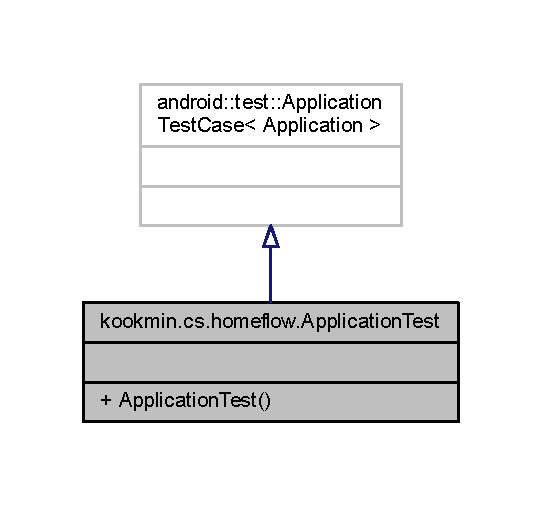
\includegraphics[width=260pt]{classkookmin_1_1cs_1_1homeflow_1_1_application_test__inherit__graph}
\end{center}
\end{figure}


kookmin.\+cs.\+homeflow.\+Application\+Test에 대한 협력 다이어그램\+:\nopagebreak
\begin{figure}[H]
\begin{center}
\leavevmode
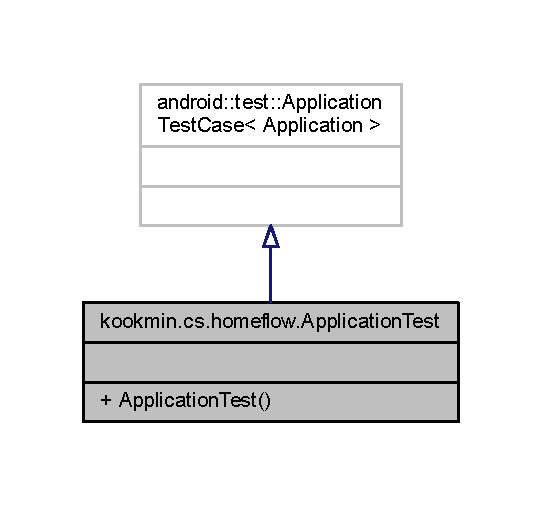
\includegraphics[width=260pt]{classkookmin_1_1cs_1_1homeflow_1_1_application_test__coll__graph}
\end{center}
\end{figure}


\subsection{상세한 설명}
\href{http://d.android.com/tools/testing/testing_android.html}{\tt Testing Fundamentals} 

이 클래스에 대한 문서화 페이지는 다음의 파일로부터 생성되었습니다.\+:\begin{DoxyCompactItemize}
\item 
D\+:/github/\+Home\+Flow/\+Androidapp/\+Home\+Flow/app/src/android\+Test/java/kookmin/cs/homeflow/Application\+Test.\+java\end{DoxyCompactItemize}

\hypertarget{classkookmin_1_1cs_1_1homeflow_1_1_dashboard_activity}{}\section{kookmin.\+cs.\+homeflow.\+Dashboard\+Activity 클래스 참조}
\label{classkookmin_1_1cs_1_1homeflow_1_1_dashboard_activity}\index{kookmin.\+cs.\+homeflow.\+Dashboard\+Activity@{kookmin.\+cs.\+homeflow.\+Dashboard\+Activity}}


an Activity is dashboard of the progress of workflow  




kookmin.\+cs.\+homeflow.\+Dashboard\+Activity에 대한 상속 다이어그램 \+: \nopagebreak
\begin{figure}[H]
\begin{center}
\leavevmode
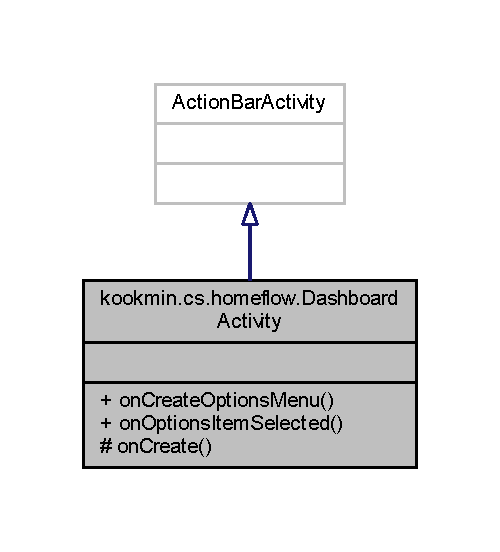
\includegraphics[width=240pt]{classkookmin_1_1cs_1_1homeflow_1_1_dashboard_activity__inherit__graph}
\end{center}
\end{figure}


kookmin.\+cs.\+homeflow.\+Dashboard\+Activity에 대한 협력 다이어그램\+:\nopagebreak
\begin{figure}[H]
\begin{center}
\leavevmode
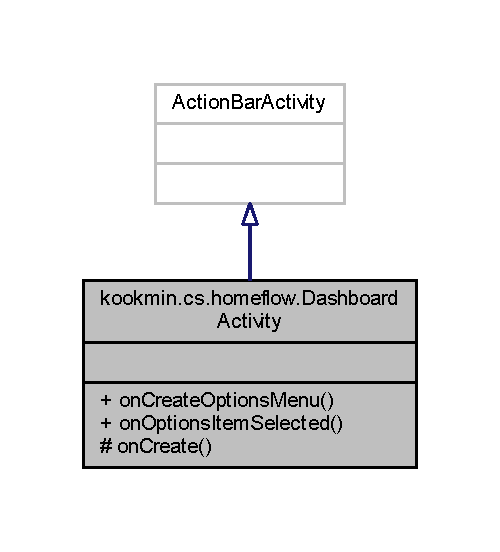
\includegraphics[width=240pt]{classkookmin_1_1cs_1_1homeflow_1_1_dashboard_activity__coll__graph}
\end{center}
\end{figure}
\subsection*{Public 멤버 함수}
\begin{DoxyCompactItemize}
\item 
\hypertarget{classkookmin_1_1cs_1_1homeflow_1_1_dashboard_activity_a0029ef83ec04c88b44dd06af1ba33552}{}boolean {\bfseries on\+Create\+Options\+Menu} (Menu menu)\label{classkookmin_1_1cs_1_1homeflow_1_1_dashboard_activity_a0029ef83ec04c88b44dd06af1ba33552}

\item 
\hypertarget{classkookmin_1_1cs_1_1homeflow_1_1_dashboard_activity_a344c2d053fb5af992768b4cac477899b}{}boolean {\bfseries on\+Options\+Item\+Selected} (Menu\+Item item)\label{classkookmin_1_1cs_1_1homeflow_1_1_dashboard_activity_a344c2d053fb5af992768b4cac477899b}

\end{DoxyCompactItemize}
\subsection*{Protected 멤버 함수}
\begin{DoxyCompactItemize}
\item 
\hypertarget{classkookmin_1_1cs_1_1homeflow_1_1_dashboard_activity_a4906b7049b563651534d0b9996e8788d}{}void {\bfseries on\+Create} (Bundle saved\+Instance\+State)\label{classkookmin_1_1cs_1_1homeflow_1_1_dashboard_activity_a4906b7049b563651534d0b9996e8788d}

\end{DoxyCompactItemize}


\subsection{상세한 설명}
an Activity is dashboard of the progress of workflow 

\begin{DoxyAuthor}{작성자}
Jongho Lim, \href{mailto:sloth@kookmin.ac.kr}{\tt sloth@kookmin.\+ac.\+kr} 

Jinsung choi, \href{mailto:bugslife102401@nate.com}{\tt bugslife102401@nate.\+com} 
\end{DoxyAuthor}
\begin{DoxyVersion}{버전}
0.\+0.\+1
\end{DoxyVersion}
workflow 의 진행상황을 보여주는 Activity Class이다. Action\+Bar의 메뉴에서 workflow edit와 device edit 등을 할 수 있다. \begin{DoxyRefDesc}{할일}
\item[\hyperlink{todo__todo000001}{할일}]Read workflow file(xml parse), check progress of workflow, etc... \end{DoxyRefDesc}


이 클래스에 대한 문서화 페이지는 다음의 파일로부터 생성되었습니다.\+:\begin{DoxyCompactItemize}
\item 
D\+:/github/\+Home\+Flow/\+Androidapp/\+Home\+Flow/app/src/main/java/kookmin/cs/homeflow/Dashboard\+Activity.\+java\end{DoxyCompactItemize}

\hypertarget{classkookmin_1_1cs_1_1homeflow_1_1data_1_1_device}{}\section{kookmin.\+cs.\+homeflow.\+data.\+Device 클래스 참조}
\label{classkookmin_1_1cs_1_1homeflow_1_1data_1_1_device}\index{kookmin.\+cs.\+homeflow.\+data.\+Device@{kookmin.\+cs.\+homeflow.\+data.\+Device}}


an Class is data of \hyperlink{classkookmin_1_1cs_1_1homeflow_1_1data_1_1_device}{Device}  




kookmin.\+cs.\+homeflow.\+data.\+Device에 대한 협력 다이어그램\+:
\nopagebreak
\begin{figure}[H]
\begin{center}
\leavevmode
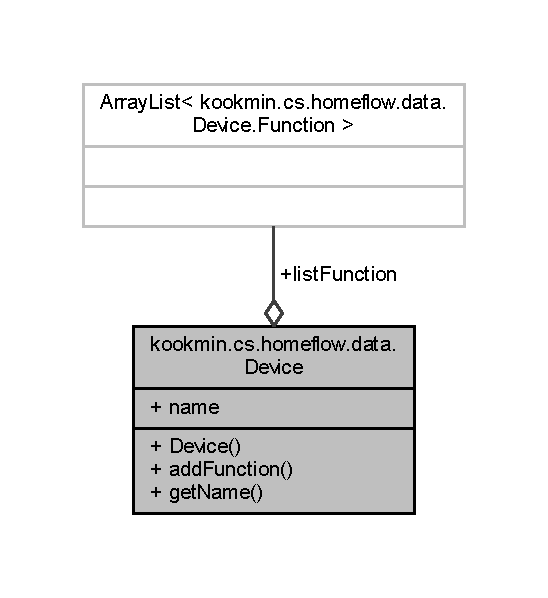
\includegraphics[width=263pt]{classkookmin_1_1cs_1_1homeflow_1_1data_1_1_device__coll__graph}
\end{center}
\end{figure}
\subsection*{클래스}
\begin{DoxyCompactItemize}
\item 
class \hyperlink{classkookmin_1_1cs_1_1homeflow_1_1data_1_1_device_1_1_function}{Function}
\begin{DoxyCompactList}\small\item\em an Class is inner class of \hyperlink{classkookmin_1_1cs_1_1homeflow_1_1data_1_1_device}{Device} class \end{DoxyCompactList}\end{DoxyCompactItemize}
\subsection*{Public 멤버 함수}
\begin{DoxyCompactItemize}
\item 
\hypertarget{classkookmin_1_1cs_1_1homeflow_1_1data_1_1_device_ad4b0feaf738c9269086530e34287742e}{}{\bfseries Device} (String device\+Name)\label{classkookmin_1_1cs_1_1homeflow_1_1data_1_1_device_ad4b0feaf738c9269086530e34287742e}

\item 
\hypertarget{classkookmin_1_1cs_1_1homeflow_1_1data_1_1_device_ad73791d1f6f6c834607febf96a913aae}{}void {\bfseries add\+Function} (\hyperlink{classkookmin_1_1cs_1_1homeflow_1_1data_1_1_device_1_1_function}{Function} func)\label{classkookmin_1_1cs_1_1homeflow_1_1data_1_1_device_ad73791d1f6f6c834607febf96a913aae}

\item 
\hypertarget{classkookmin_1_1cs_1_1homeflow_1_1data_1_1_device_a33ea9a154660683d27f9ad6dfc274727}{}String {\bfseries get\+Name} ()\label{classkookmin_1_1cs_1_1homeflow_1_1data_1_1_device_a33ea9a154660683d27f9ad6dfc274727}

\end{DoxyCompactItemize}
\subsection*{Public 속성}
\begin{DoxyCompactItemize}
\item 
\hypertarget{classkookmin_1_1cs_1_1homeflow_1_1data_1_1_device_aa73d606e01900b24374b07ec6b063032}{}String {\bfseries name}\label{classkookmin_1_1cs_1_1homeflow_1_1data_1_1_device_aa73d606e01900b24374b07ec6b063032}

\item 
\hypertarget{classkookmin_1_1cs_1_1homeflow_1_1data_1_1_device_ab677ca512cac1353c961757d9870775e}{}Array\+List$<$ \hyperlink{classkookmin_1_1cs_1_1homeflow_1_1data_1_1_device_1_1_function}{Function} $>$ {\bfseries list\+Function}\label{classkookmin_1_1cs_1_1homeflow_1_1data_1_1_device_ab677ca512cac1353c961757d9870775e}

\end{DoxyCompactItemize}


\subsection{상세한 설명}
an Class is data of \hyperlink{classkookmin_1_1cs_1_1homeflow_1_1data_1_1_device}{Device} 

\begin{DoxyAuthor}{작성자}
Jongho Lim, \href{mailto:sloth@kookmin.ac.kr}{\tt sloth@kookmin.\+ac.\+kr} 

Jinsung choi, \href{mailto:bugslife102401@nate.com}{\tt bugslife102401@nate.\+com} 
\end{DoxyAuthor}
\begin{DoxyVersion}{버전}
0.\+0.\+1
\end{DoxyVersion}
Device의 data를 가지고 있는 class이다. device의 이름과 기능들의 리스트를 담고 있다. 

이 클래스에 대한 문서화 페이지는 다음의 파일로부터 생성되었습니다.\+:\begin{DoxyCompactItemize}
\item 
D\+:/github/\+Home\+Flow/\+Androidapp/\+Home\+Flow/app/src/main/java/kookmin/cs/homeflow/data/Device.\+java\end{DoxyCompactItemize}

\hypertarget{classkookmin_1_1cs_1_1homeflow_1_1_device_list_activity}{}\section{kookmin.\+cs.\+homeflow.\+Device\+List\+Activity 클래스 참조}
\label{classkookmin_1_1cs_1_1homeflow_1_1_device_list_activity}\index{kookmin.\+cs.\+homeflow.\+Device\+List\+Activity@{kookmin.\+cs.\+homeflow.\+Device\+List\+Activity}}


an Activity is show device and able to function  




kookmin.\+cs.\+homeflow.\+Device\+List\+Activity에 대한 상속 다이어그램 \+: \nopagebreak
\begin{figure}[H]
\begin{center}
\leavevmode
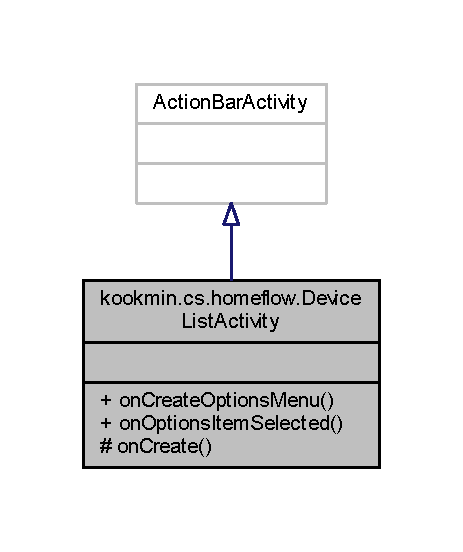
\includegraphics[width=222pt]{classkookmin_1_1cs_1_1homeflow_1_1_device_list_activity__inherit__graph}
\end{center}
\end{figure}


kookmin.\+cs.\+homeflow.\+Device\+List\+Activity에 대한 협력 다이어그램\+:\nopagebreak
\begin{figure}[H]
\begin{center}
\leavevmode
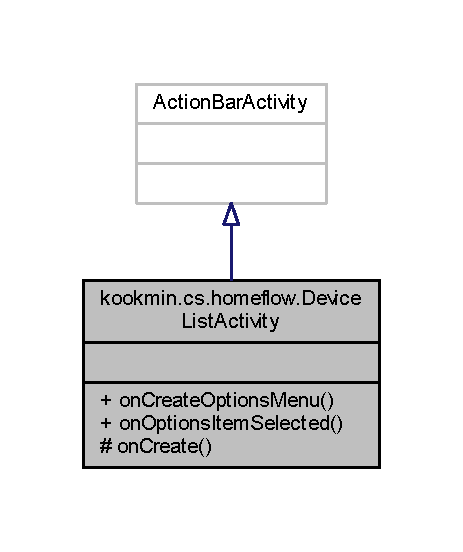
\includegraphics[width=222pt]{classkookmin_1_1cs_1_1homeflow_1_1_device_list_activity__coll__graph}
\end{center}
\end{figure}
\subsection*{Public 멤버 함수}
\begin{DoxyCompactItemize}
\item 
\hypertarget{classkookmin_1_1cs_1_1homeflow_1_1_device_list_activity_a24518f31fe0724be786fc7682a077d9d}{}boolean {\bfseries on\+Create\+Options\+Menu} (Menu menu)\label{classkookmin_1_1cs_1_1homeflow_1_1_device_list_activity_a24518f31fe0724be786fc7682a077d9d}

\item 
\hypertarget{classkookmin_1_1cs_1_1homeflow_1_1_device_list_activity_aa9cced735407297a166b944d58b4f416}{}boolean {\bfseries on\+Options\+Item\+Selected} (Menu\+Item item)\label{classkookmin_1_1cs_1_1homeflow_1_1_device_list_activity_aa9cced735407297a166b944d58b4f416}

\end{DoxyCompactItemize}
\subsection*{Protected 멤버 함수}
\begin{DoxyCompactItemize}
\item 
\hypertarget{classkookmin_1_1cs_1_1homeflow_1_1_device_list_activity_a22ce55d384f34491240185b26126007b}{}void {\bfseries on\+Create} (Bundle saved\+Instance\+State)\label{classkookmin_1_1cs_1_1homeflow_1_1_device_list_activity_a22ce55d384f34491240185b26126007b}

\end{DoxyCompactItemize}


\subsection{상세한 설명}
an Activity is show device and able to function 

\begin{DoxyAuthor}{작성자}
Jongho Lim, \href{mailto:sloth@kookmin.ac.kr}{\tt sloth@kookmin.\+ac.\+kr} 

Jinsung choi, \href{mailto:bugslife102401@nate.com}{\tt bugslife102401@nate.\+com} 
\end{DoxyAuthor}
\begin{DoxyVersion}{버전}
0.\+0.\+1
\end{DoxyVersion}
현재 등록된 appliance와 사용 가능한 appliance의 기능이 나온다. \begin{DoxyRefDesc}{할일}
\item[\hyperlink{todo__todo000002}{할일}]develop ... \end{DoxyRefDesc}


이 클래스에 대한 문서화 페이지는 다음의 파일로부터 생성되었습니다.\+:\begin{DoxyCompactItemize}
\item 
D\+:/github/\+Home\+Flow/\+Androidapp/\+Home\+Flow/app/src/main/java/kookmin/cs/homeflow/Device\+List\+Activity.\+java\end{DoxyCompactItemize}

\hypertarget{classkookmin_1_1cs_1_1homeflow_1_1_flow_list_activity}{}\section{kookmin.\+cs.\+homeflow.\+Flow\+List\+Activity 클래스 참조}
\label{classkookmin_1_1cs_1_1homeflow_1_1_flow_list_activity}\index{kookmin.\+cs.\+homeflow.\+Flow\+List\+Activity@{kookmin.\+cs.\+homeflow.\+Flow\+List\+Activity}}


an Activity is show workflow list existent(able to edit)  




kookmin.\+cs.\+homeflow.\+Flow\+List\+Activity에 대한 상속 다이어그램 \+: \nopagebreak
\begin{figure}[H]
\begin{center}
\leavevmode
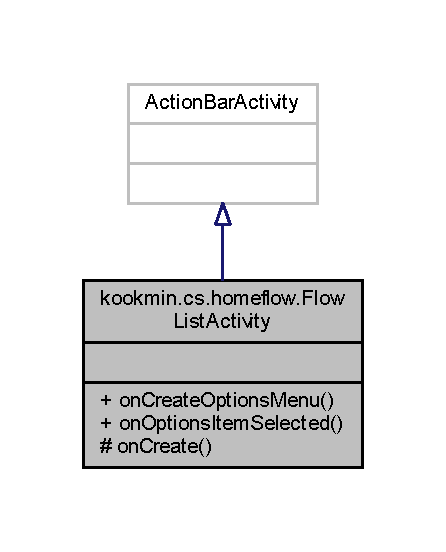
\includegraphics[width=214pt]{classkookmin_1_1cs_1_1homeflow_1_1_flow_list_activity__inherit__graph}
\end{center}
\end{figure}


kookmin.\+cs.\+homeflow.\+Flow\+List\+Activity에 대한 협력 다이어그램\+:\nopagebreak
\begin{figure}[H]
\begin{center}
\leavevmode
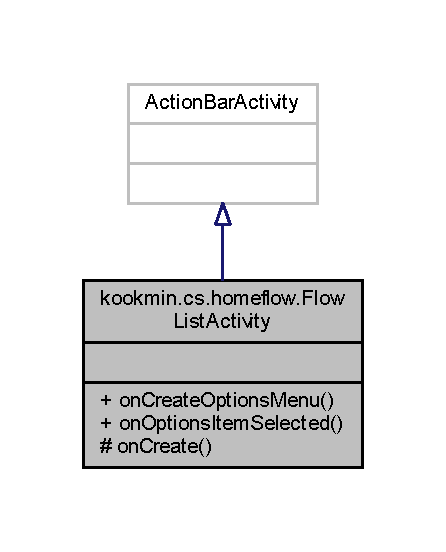
\includegraphics[width=214pt]{classkookmin_1_1cs_1_1homeflow_1_1_flow_list_activity__coll__graph}
\end{center}
\end{figure}
\subsection*{Public 멤버 함수}
\begin{DoxyCompactItemize}
\item 
\hypertarget{classkookmin_1_1cs_1_1homeflow_1_1_flow_list_activity_aeefaa220dea7d250602e4e1c4dfff848}{}boolean {\bfseries on\+Create\+Options\+Menu} (Menu menu)\label{classkookmin_1_1cs_1_1homeflow_1_1_flow_list_activity_aeefaa220dea7d250602e4e1c4dfff848}

\item 
\hypertarget{classkookmin_1_1cs_1_1homeflow_1_1_flow_list_activity_a7a81313dcc21b5d7abc65d93432a9a99}{}boolean {\bfseries on\+Options\+Item\+Selected} (Menu\+Item item)\label{classkookmin_1_1cs_1_1homeflow_1_1_flow_list_activity_a7a81313dcc21b5d7abc65d93432a9a99}

\end{DoxyCompactItemize}
\subsection*{Protected 멤버 함수}
\begin{DoxyCompactItemize}
\item 
void \hyperlink{classkookmin_1_1cs_1_1homeflow_1_1_flow_list_activity_a8e7f4c315f0498cbb846022ddd0df21e}{on\+Create} (Bundle saved\+Instance\+State)
\begin{DoxyCompactList}\small\item\em Activity init. \end{DoxyCompactList}\end{DoxyCompactItemize}


\subsection{상세한 설명}
an Activity is show workflow list existent(able to edit) 

\begin{DoxyAuthor}{작성자}
Jongho Lim, \href{mailto:sloth@kookmin.ac.kr}{\tt sloth@kookmin.\+ac.\+kr} 

Jinsung choi, \href{mailto:bugslife102401@nate.com}{\tt bugslife102401@nate.\+com} 
\end{DoxyAuthor}
\begin{DoxyVersion}{버전}
0.\+0.\+3
\end{DoxyVersion}
현재 등록된 workflow의 list를 보여준다. workflow를 새로 만들수 있는 Button이 있고 list를 클릭하면 workflow를 수정 또는 삭제할 수 있다. \begin{DoxyRefDesc}{할일}
\item[\hyperlink{todo__todo000003}{할일}]develop U\+I, List Item Click, Button Click etc... \end{DoxyRefDesc}


\subsection{멤버 함수 문서화}
\hypertarget{classkookmin_1_1cs_1_1homeflow_1_1_flow_list_activity_a8e7f4c315f0498cbb846022ddd0df21e}{}\index{kookmin\+::cs\+::homeflow\+::\+Flow\+List\+Activity@{kookmin\+::cs\+::homeflow\+::\+Flow\+List\+Activity}!on\+Create@{on\+Create}}
\index{on\+Create@{on\+Create}!kookmin\+::cs\+::homeflow\+::\+Flow\+List\+Activity@{kookmin\+::cs\+::homeflow\+::\+Flow\+List\+Activity}}
\subsubsection[{on\+Create}]{\setlength{\rightskip}{0pt plus 5cm}void kookmin.\+cs.\+homeflow.\+Flow\+List\+Activity.\+on\+Create (
\begin{DoxyParamCaption}
\item[{Bundle}]{saved\+Instance\+State}
\end{DoxyParamCaption}
)\hspace{0.3cm}{\ttfamily [protected]}}\label{classkookmin_1_1cs_1_1homeflow_1_1_flow_list_activity_a8e7f4c315f0498cbb846022ddd0df21e}


Activity init. 

Activity를 init한다. 데이터를 listview로 보여준다. listview의 속성을 변경한다. \begin{DoxyRefDesc}{할일}
\item[\hyperlink{todo__todo000004}{할일}]read list of workflow xml file and show \end{DoxyRefDesc}

\begin{DoxyCode}
36                                                      \{
37     super.onCreate(savedInstanceState);
38     setContentView(R.layout.activity\_workflow\_list);
39 
40     getSupportActionBar().setTitle(\textcolor{stringliteral}{"FlowList"});
41     \textcolor{comment}{// set data}
42     ArrayList<String> dashlist = \textcolor{keyword}{new} ArrayList<String>();
43 
44     dashlist.add(\textcolor{stringliteral}{"세탁기 workflow"});
45     dashlist.add(\textcolor{stringliteral}{"집 나갈때 workflow"});
46     dashlist.add(\textcolor{stringliteral}{"잠 자기 전 workflow"});
47 
48     \textcolor{comment}{// set adapter}
49     ArrayAdapter<String> adapter;
50     adapter =
51         \textcolor{keyword}{new} ArrayAdapter<String>(\textcolor{keyword}{this}, android.R.layout.simple\_expandable\_list\_item\_1, dashlist);
52 
53     \textcolor{comment}{// connect adapter}
54     ListView list = (ListView) findViewById(R.id.dash\_list);
55     list.setAdapter(adapter);
56 
57     \textcolor{comment}{// ListView attribute}
58     list.setChoiceMode(ListView.CHOICE\_MODE\_SINGLE);
59     list.setDivider(\textcolor{keyword}{new} ColorDrawable(Color.WHITE));
60     list.setDividerHeight(2);
61   \}
\end{DoxyCode}


이 클래스에 대한 문서화 페이지는 다음의 파일로부터 생성되었습니다.\+:\begin{DoxyCompactItemize}
\item 
D\+:/github/\+Home\+Flow/\+Androidapp/\+Home\+Flow/app/src/main/java/kookmin/cs/homeflow/Flow\+List\+Activity.\+java\end{DoxyCompactItemize}

\hypertarget{classkookmin_1_1cs_1_1homeflow_1_1data_1_1_device_1_1_function}{}\section{kookmin.\+cs.\+homeflow.\+data.\+Device.\+Function 클래스 참조}
\label{classkookmin_1_1cs_1_1homeflow_1_1data_1_1_device_1_1_function}\index{kookmin.\+cs.\+homeflow.\+data.\+Device.\+Function@{kookmin.\+cs.\+homeflow.\+data.\+Device.\+Function}}


an Class is inner class of \hyperlink{classkookmin_1_1cs_1_1homeflow_1_1data_1_1_device}{Device} class  




kookmin.\+cs.\+homeflow.\+data.\+Device.\+Function에 대한 협력 다이어그램\+:
\nopagebreak
\begin{figure}[H]
\begin{center}
\leavevmode
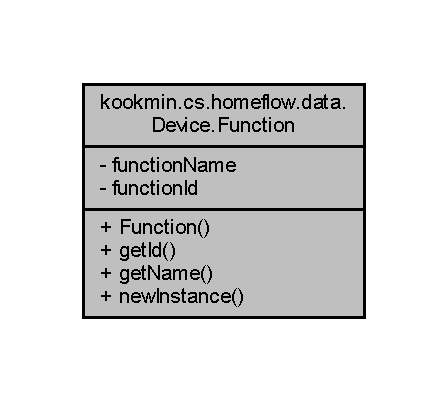
\includegraphics[width=215pt]{classkookmin_1_1cs_1_1homeflow_1_1data_1_1_device_1_1_function__coll__graph}
\end{center}
\end{figure}
\subsection*{Public 멤버 함수}
\begin{DoxyCompactItemize}
\item 
\hypertarget{classkookmin_1_1cs_1_1homeflow_1_1data_1_1_device_1_1_function_ae4fe76146719f7d0ff2f5b610b49eca3}{}{\bfseries Function} (String func\+Name, int func\+Id)\label{classkookmin_1_1cs_1_1homeflow_1_1data_1_1_device_1_1_function_ae4fe76146719f7d0ff2f5b610b49eca3}

\item 
\hypertarget{classkookmin_1_1cs_1_1homeflow_1_1data_1_1_device_1_1_function_ad824c47111de83b319140b7ee85209bd}{}int {\bfseries get\+Id} ()\label{classkookmin_1_1cs_1_1homeflow_1_1data_1_1_device_1_1_function_ad824c47111de83b319140b7ee85209bd}

\item 
\hypertarget{classkookmin_1_1cs_1_1homeflow_1_1data_1_1_device_1_1_function_a7b41f1357734eb854ac3500a596d4795}{}String {\bfseries get\+Name} ()\label{classkookmin_1_1cs_1_1homeflow_1_1data_1_1_device_1_1_function_a7b41f1357734eb854ac3500a596d4795}

\end{DoxyCompactItemize}
\subsection*{정적 Public 멤버 함수}
\begin{DoxyCompactItemize}
\item 
\hypertarget{classkookmin_1_1cs_1_1homeflow_1_1data_1_1_device_1_1_function_a0ed84ea09c81e6b8815ec91d9045a057}{}static \hyperlink{classkookmin_1_1cs_1_1homeflow_1_1data_1_1_device_1_1_function}{Function} {\bfseries new\+Instance} (String func\+Name, int func\+Id)\label{classkookmin_1_1cs_1_1homeflow_1_1data_1_1_device_1_1_function_a0ed84ea09c81e6b8815ec91d9045a057}

\end{DoxyCompactItemize}
\subsection*{Private 속성}
\begin{DoxyCompactItemize}
\item 
\hypertarget{classkookmin_1_1cs_1_1homeflow_1_1data_1_1_device_1_1_function_a5321ffa1136b94b8727d23a44de8e397}{}String {\bfseries function\+Name}\label{classkookmin_1_1cs_1_1homeflow_1_1data_1_1_device_1_1_function_a5321ffa1136b94b8727d23a44de8e397}

\item 
\hypertarget{classkookmin_1_1cs_1_1homeflow_1_1data_1_1_device_1_1_function_a6f9bff7543180a9232c102c7169b8308}{}int {\bfseries function\+Id}\label{classkookmin_1_1cs_1_1homeflow_1_1data_1_1_device_1_1_function_a6f9bff7543180a9232c102c7169b8308}

\end{DoxyCompactItemize}


\subsection{상세한 설명}
an Class is inner class of \hyperlink{classkookmin_1_1cs_1_1homeflow_1_1data_1_1_device}{Device} class 

\begin{DoxyAuthor}{작성자}
Jongho Lim, \href{mailto:sloth@kookmin.ac.kr}{\tt sloth@kookmin.\+ac.\+kr} 

Jinsung choi, \href{mailto:bugslife102401@nate.com}{\tt bugslife102401@nate.\+com} 
\end{DoxyAuthor}
\begin{DoxyVersion}{버전}
0.\+0.\+1
\end{DoxyVersion}
\hyperlink{classkookmin_1_1cs_1_1homeflow_1_1data_1_1_device}{Device} class 의 inner class이다. Device의 기능들을 담을 수 있다. 

이 클래스에 대한 문서화 페이지는 다음의 파일로부터 생성되었습니다.\+:\begin{DoxyCompactItemize}
\item 
D\+:/github/\+Home\+Flow/\+Androidapp/\+Home\+Flow/app/src/main/java/kookmin/cs/homeflow/data/Device.\+java\end{DoxyCompactItemize}

\hypertarget{classkookmin_1_1cs_1_1homeflow_1_1_login_activity}{}\section{kookmin.\+cs.\+homeflow.\+Login\+Activity 클래스 참조}
\label{classkookmin_1_1cs_1_1homeflow_1_1_login_activity}\index{kookmin.\+cs.\+homeflow.\+Login\+Activity@{kookmin.\+cs.\+homeflow.\+Login\+Activity}}


an Activity for Login  




kookmin.\+cs.\+homeflow.\+Login\+Activity에 대한 상속 다이어그램 \+: \nopagebreak
\begin{figure}[H]
\begin{center}
\leavevmode
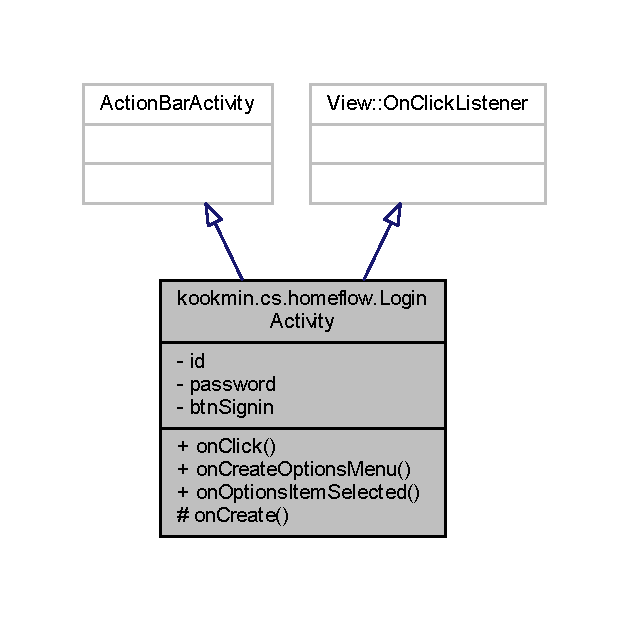
\includegraphics[width=302pt]{classkookmin_1_1cs_1_1homeflow_1_1_login_activity__inherit__graph}
\end{center}
\end{figure}


kookmin.\+cs.\+homeflow.\+Login\+Activity에 대한 협력 다이어그램\+:\nopagebreak
\begin{figure}[H]
\begin{center}
\leavevmode
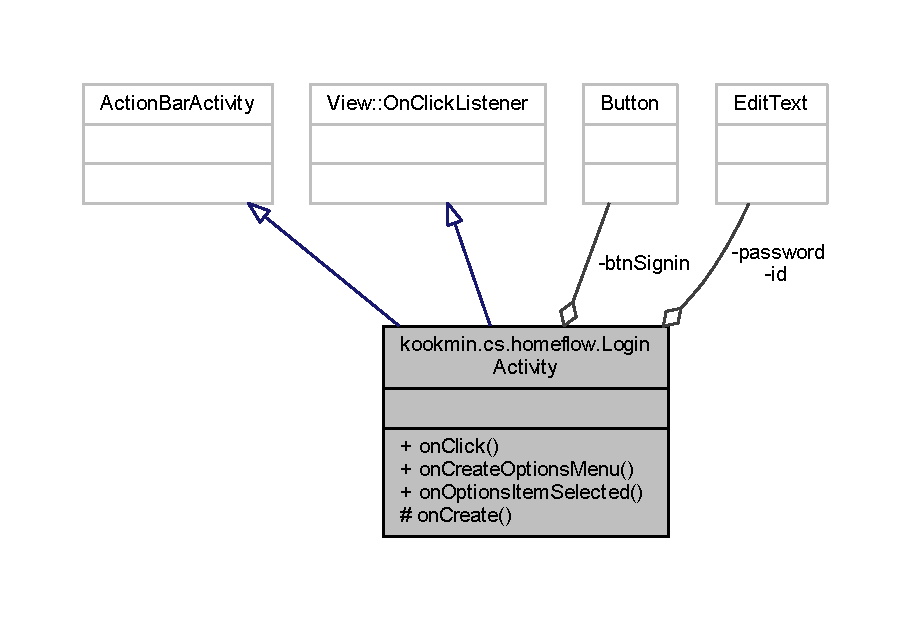
\includegraphics[width=350pt]{classkookmin_1_1cs_1_1homeflow_1_1_login_activity__coll__graph}
\end{center}
\end{figure}
\subsection*{Public 멤버 함수}
\begin{DoxyCompactItemize}
\item 
void \hyperlink{classkookmin_1_1cs_1_1homeflow_1_1_login_activity_a29cfa7fedc97be0ec337678df698100f}{on\+Click} (View v)
\begin{DoxyCompactList}\small\item\em process click event \end{DoxyCompactList}\item 
\hypertarget{classkookmin_1_1cs_1_1homeflow_1_1_login_activity_aaf30dacb9b1247a33814d92f94c6a47d}{}boolean {\bfseries on\+Create\+Options\+Menu} (Menu menu)\label{classkookmin_1_1cs_1_1homeflow_1_1_login_activity_aaf30dacb9b1247a33814d92f94c6a47d}

\item 
\hypertarget{classkookmin_1_1cs_1_1homeflow_1_1_login_activity_a1030ae5e1d39703ce27b03a3644627f9}{}boolean {\bfseries on\+Options\+Item\+Selected} (Menu\+Item item)\label{classkookmin_1_1cs_1_1homeflow_1_1_login_activity_a1030ae5e1d39703ce27b03a3644627f9}

\end{DoxyCompactItemize}
\subsection*{Protected 멤버 함수}
\begin{DoxyCompactItemize}
\item 
void \hyperlink{classkookmin_1_1cs_1_1homeflow_1_1_login_activity_af4c64a06bcf604e369c9d4af370d4951}{on\+Create} (Bundle saved\+Instance\+State)
\begin{DoxyCompactList}\small\item\em Activity init. \end{DoxyCompactList}\end{DoxyCompactItemize}
\subsection*{Private 속성}
\begin{DoxyCompactItemize}
\item 
\hypertarget{classkookmin_1_1cs_1_1homeflow_1_1_login_activity_ac9268855aae891b4b9dae821e2f1e158}{}Edit\+Text {\bfseries id}\label{classkookmin_1_1cs_1_1homeflow_1_1_login_activity_ac9268855aae891b4b9dae821e2f1e158}

\item 
\hypertarget{classkookmin_1_1cs_1_1homeflow_1_1_login_activity_ab6d1fac18412c27ecf94293ed1f28055}{}Edit\+Text {\bfseries password}\label{classkookmin_1_1cs_1_1homeflow_1_1_login_activity_ab6d1fac18412c27ecf94293ed1f28055}

\item 
\hypertarget{classkookmin_1_1cs_1_1homeflow_1_1_login_activity_a6d09cf9476263a19cb6ed6342d4de60c}{}Button {\bfseries btn\+Signin}\label{classkookmin_1_1cs_1_1homeflow_1_1_login_activity_a6d09cf9476263a19cb6ed6342d4de60c}

\end{DoxyCompactItemize}


\subsection{상세한 설명}
an Activity for Login 

\begin{DoxyAuthor}{작성자}
Jongho Lim, \href{mailto:sloth@kookmin.ac.kr}{\tt sloth@kookmin.\+ac.\+kr} 

Jinsung choi, \href{mailto:bugslife102401@nate.com}{\tt bugslife102401@nate.\+com} 
\end{DoxyAuthor}
\begin{DoxyVersion}{버전}
0.\+0.\+1
\end{DoxyVersion}
Action\+Bar를 가지고있고 Login 기능을 지원하는 Activity Class이다. U\+I로는 id와 password를 적을 수 있는 Edit\+Text 가 두 개 있고 sign in(login) 기능을 지원하는 Button이 한 개 있다. \begin{DoxyRefDesc}{할일}
\item[\hyperlink{todo__todo000005}{할일}]function develop user check with server communication \end{DoxyRefDesc}


\subsection{멤버 함수 문서화}
\hypertarget{classkookmin_1_1cs_1_1homeflow_1_1_login_activity_a29cfa7fedc97be0ec337678df698100f}{}\index{kookmin\+::cs\+::homeflow\+::\+Login\+Activity@{kookmin\+::cs\+::homeflow\+::\+Login\+Activity}!on\+Click@{on\+Click}}
\index{on\+Click@{on\+Click}!kookmin\+::cs\+::homeflow\+::\+Login\+Activity@{kookmin\+::cs\+::homeflow\+::\+Login\+Activity}}
\subsubsection[{on\+Click}]{\setlength{\rightskip}{0pt plus 5cm}void kookmin.\+cs.\+homeflow.\+Login\+Activity.\+on\+Click (
\begin{DoxyParamCaption}
\item[{View}]{v}
\end{DoxyParamCaption}
)}\label{classkookmin_1_1cs_1_1homeflow_1_1_login_activity_a29cfa7fedc97be0ec337678df698100f}


process click event 


\begin{DoxyParams}{매개변수}
{\em v} & clicked view\\
\hline
\end{DoxyParams}
Sign in Button이 클릭되면 실행되는 method이다. 사용자가 확인 되면 Dash\+Board Activity로 넘어간다. \begin{DoxyRefDesc}{할일}
\item[\hyperlink{todo__todo000006}{할일}]implement function user check with server communication \end{DoxyRefDesc}

\begin{DoxyCode}
55                               \{
56     \textcolor{keywordflow}{switch} (v.getId()) \{
57       \textcolor{keywordflow}{case} R.id.btnSignin:
58         startActivity(\textcolor{keyword}{new} Intent(LoginActivity.this, DashboardActivity.class));
59         finish();
60         \textcolor{keywordflow}{break};
61     \}
62   \}
\end{DoxyCode}
\hypertarget{classkookmin_1_1cs_1_1homeflow_1_1_login_activity_af4c64a06bcf604e369c9d4af370d4951}{}\index{kookmin\+::cs\+::homeflow\+::\+Login\+Activity@{kookmin\+::cs\+::homeflow\+::\+Login\+Activity}!on\+Create@{on\+Create}}
\index{on\+Create@{on\+Create}!kookmin\+::cs\+::homeflow\+::\+Login\+Activity@{kookmin\+::cs\+::homeflow\+::\+Login\+Activity}}
\subsubsection[{on\+Create}]{\setlength{\rightskip}{0pt plus 5cm}void kookmin.\+cs.\+homeflow.\+Login\+Activity.\+on\+Create (
\begin{DoxyParamCaption}
\item[{Bundle}]{saved\+Instance\+State}
\end{DoxyParamCaption}
)\hspace{0.3cm}{\ttfamily [protected]}}\label{classkookmin_1_1cs_1_1homeflow_1_1_login_activity_af4c64a06bcf604e369c9d4af370d4951}


Activity init. 

Edit\+Text와 Button을 init 시키고 Button에 click event를 등록한다. 
\begin{DoxyCode}
37                                                      \{
38     super.onCreate(savedInstanceState);
39     setContentView(R.layout.activity\_login);
40 
41     \textcolor{keywordtype}{id} = (EditText) findViewById(R.id.editId);
42     password = (EditText) findViewById(R.id.editPwd);
43     btnSignin = (Button) findViewById(R.id.btnSignin);
44 
45     btnSignin.setOnClickListener(\textcolor{keyword}{this});
46   \}
\end{DoxyCode}


이 클래스에 대한 문서화 페이지는 다음의 파일로부터 생성되었습니다.\+:\begin{DoxyCompactItemize}
\item 
D\+:/github/\+Home\+Flow/\+Androidapp/\+Home\+Flow/app/src/main/java/kookmin/cs/homeflow/Login\+Activity.\+java\end{DoxyCompactItemize}

\hypertarget{classkookmin_1_1cs_1_1homeflow_1_1data_1_1_workflow_1_1_work}{}\section{kookmin.\+cs.\+homeflow.\+data.\+Workflow.\+Work 클래스 참조}
\label{classkookmin_1_1cs_1_1homeflow_1_1data_1_1_workflow_1_1_work}\index{kookmin.\+cs.\+homeflow.\+data.\+Workflow.\+Work@{kookmin.\+cs.\+homeflow.\+data.\+Workflow.\+Work}}


an Class is inner class of \hyperlink{classkookmin_1_1cs_1_1homeflow_1_1data_1_1_workflow}{Workflow} class  




kookmin.\+cs.\+homeflow.\+data.\+Workflow.\+Work에 대한 협력 다이어그램\+:
\nopagebreak
\begin{figure}[H]
\begin{center}
\leavevmode
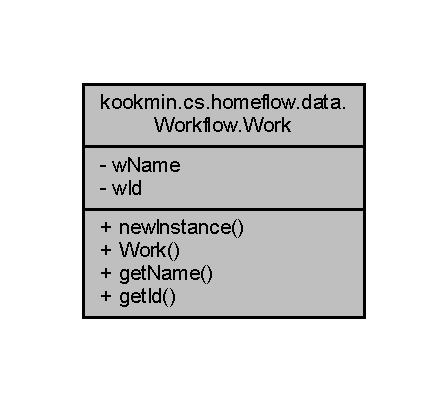
\includegraphics[width=215pt]{classkookmin_1_1cs_1_1homeflow_1_1data_1_1_workflow_1_1_work__coll__graph}
\end{center}
\end{figure}
\subsection*{Public 멤버 함수}
\begin{DoxyCompactItemize}
\item 
\hypertarget{classkookmin_1_1cs_1_1homeflow_1_1data_1_1_workflow_1_1_work_afe3587469c681483da0b2881fe2b03bd}{}\hyperlink{classkookmin_1_1cs_1_1homeflow_1_1data_1_1_workflow_1_1_work}{Work} {\bfseries new\+Instance} (String work\+Name, int work\+Id)\label{classkookmin_1_1cs_1_1homeflow_1_1data_1_1_workflow_1_1_work_afe3587469c681483da0b2881fe2b03bd}

\item 
\hypertarget{classkookmin_1_1cs_1_1homeflow_1_1data_1_1_workflow_1_1_work_a884e351e82d281343e03cc90d9dab30a}{}{\bfseries Work} (String work\+Name, int work\+Id)\label{classkookmin_1_1cs_1_1homeflow_1_1data_1_1_workflow_1_1_work_a884e351e82d281343e03cc90d9dab30a}

\item 
\hypertarget{classkookmin_1_1cs_1_1homeflow_1_1data_1_1_workflow_1_1_work_afe184c07ba88058ba213fc98e1f85375}{}String {\bfseries get\+Name} ()\label{classkookmin_1_1cs_1_1homeflow_1_1data_1_1_workflow_1_1_work_afe184c07ba88058ba213fc98e1f85375}

\item 
\hypertarget{classkookmin_1_1cs_1_1homeflow_1_1data_1_1_workflow_1_1_work_aea5128d4e754d459b8ca05fc5b866194}{}int {\bfseries get\+Id} ()\label{classkookmin_1_1cs_1_1homeflow_1_1data_1_1_workflow_1_1_work_aea5128d4e754d459b8ca05fc5b866194}

\end{DoxyCompactItemize}
\subsection*{Private 속성}
\begin{DoxyCompactItemize}
\item 
\hypertarget{classkookmin_1_1cs_1_1homeflow_1_1data_1_1_workflow_1_1_work_ad3f6072bc6ef8d0b20def5a61a93d7e7}{}String {\bfseries w\+Name}\label{classkookmin_1_1cs_1_1homeflow_1_1data_1_1_workflow_1_1_work_ad3f6072bc6ef8d0b20def5a61a93d7e7}

\item 
\hypertarget{classkookmin_1_1cs_1_1homeflow_1_1data_1_1_workflow_1_1_work_abd2d4f235e90c1b2e51c16d211cd6f5e}{}int {\bfseries w\+Id}\label{classkookmin_1_1cs_1_1homeflow_1_1data_1_1_workflow_1_1_work_abd2d4f235e90c1b2e51c16d211cd6f5e}

\end{DoxyCompactItemize}


\subsection{상세한 설명}
an Class is inner class of \hyperlink{classkookmin_1_1cs_1_1homeflow_1_1data_1_1_workflow}{Workflow} class 

\begin{DoxyAuthor}{작성자}
Jongho Lim, \href{mailto:sloth@kookmin.ac.kr}{\tt sloth@kookmin.\+ac.\+kr} 

Jinsung choi, \href{mailto:bugslife102401@nate.com}{\tt bugslife102401@nate.\+com} 
\end{DoxyAuthor}
\begin{DoxyVersion}{버전}
0.\+0.\+1
\end{DoxyVersion}
\hyperlink{classkookmin_1_1cs_1_1homeflow_1_1data_1_1_workflow}{Workflow} class 의 inner class이다. workflow 의 각 각의 work를 담을 수 있다. 

이 클래스에 대한 문서화 페이지는 다음의 파일로부터 생성되었습니다.\+:\begin{DoxyCompactItemize}
\item 
D\+:/github/\+Home\+Flow/\+Androidapp/\+Home\+Flow/app/src/main/java/kookmin/cs/homeflow/data/Workflow.\+java\end{DoxyCompactItemize}

\hypertarget{classkookmin_1_1cs_1_1homeflow_1_1data_1_1_workflow}{}\section{kookmin.\+cs.\+homeflow.\+data.\+Workflow 클래스 참조}
\label{classkookmin_1_1cs_1_1homeflow_1_1data_1_1_workflow}\index{kookmin.\+cs.\+homeflow.\+data.\+Workflow@{kookmin.\+cs.\+homeflow.\+data.\+Workflow}}


an Class is data of workflow  




kookmin.\+cs.\+homeflow.\+data.\+Workflow에 대한 협력 다이어그램\+:
\nopagebreak
\begin{figure}[H]
\begin{center}
\leavevmode
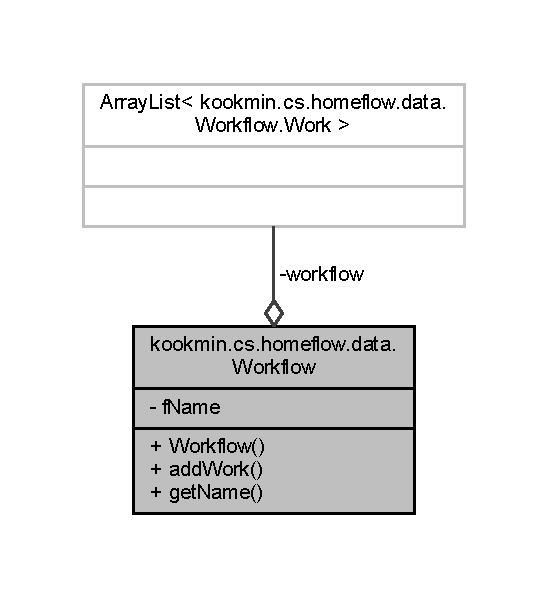
\includegraphics[width=263pt]{classkookmin_1_1cs_1_1homeflow_1_1data_1_1_workflow__coll__graph}
\end{center}
\end{figure}
\subsection*{클래스}
\begin{DoxyCompactItemize}
\item 
class \hyperlink{classkookmin_1_1cs_1_1homeflow_1_1data_1_1_workflow_1_1_work}{Work}
\begin{DoxyCompactList}\small\item\em an Class is inner class of \hyperlink{classkookmin_1_1cs_1_1homeflow_1_1data_1_1_workflow}{Workflow} class \end{DoxyCompactList}\end{DoxyCompactItemize}
\subsection*{Public 멤버 함수}
\begin{DoxyCompactItemize}
\item 
\hypertarget{classkookmin_1_1cs_1_1homeflow_1_1data_1_1_workflow_a12a9629721814a6d14c3fc4944576185}{}{\bfseries Workflow} (String flow\+Name)\label{classkookmin_1_1cs_1_1homeflow_1_1data_1_1_workflow_a12a9629721814a6d14c3fc4944576185}

\item 
\hypertarget{classkookmin_1_1cs_1_1homeflow_1_1data_1_1_workflow_a26090da91ab289560143a25063a9fd0e}{}void {\bfseries add\+Work} (\hyperlink{classkookmin_1_1cs_1_1homeflow_1_1data_1_1_workflow_1_1_work}{Work} work)\label{classkookmin_1_1cs_1_1homeflow_1_1data_1_1_workflow_a26090da91ab289560143a25063a9fd0e}

\item 
\hypertarget{classkookmin_1_1cs_1_1homeflow_1_1data_1_1_workflow_ae52da38b041aa0bb66ead165b6e88082}{}String {\bfseries get\+Name} ()\label{classkookmin_1_1cs_1_1homeflow_1_1data_1_1_workflow_ae52da38b041aa0bb66ead165b6e88082}

\end{DoxyCompactItemize}
\subsection*{Private 속성}
\begin{DoxyCompactItemize}
\item 
\hypertarget{classkookmin_1_1cs_1_1homeflow_1_1data_1_1_workflow_a73b794c2949c966cad5e34edb2249dbe}{}String {\bfseries f\+Name}\label{classkookmin_1_1cs_1_1homeflow_1_1data_1_1_workflow_a73b794c2949c966cad5e34edb2249dbe}

\item 
\hypertarget{classkookmin_1_1cs_1_1homeflow_1_1data_1_1_workflow_aa2201c9f62856d58e534199e244f1656}{}Array\+List$<$ \hyperlink{classkookmin_1_1cs_1_1homeflow_1_1data_1_1_workflow_1_1_work}{Work} $>$ {\bfseries workflow}\label{classkookmin_1_1cs_1_1homeflow_1_1data_1_1_workflow_aa2201c9f62856d58e534199e244f1656}

\end{DoxyCompactItemize}


\subsection{상세한 설명}
an Class is data of workflow 

\begin{DoxyAuthor}{작성자}
Jongho Lim, \href{mailto:sloth@kookmin.ac.kr}{\tt sloth@kookmin.\+ac.\+kr} 

Jinsung choi, \href{mailto:bugslife102401@nate.com}{\tt bugslife102401@nate.\+com} 
\end{DoxyAuthor}
\begin{DoxyVersion}{버전}
0.\+0.\+1
\end{DoxyVersion}
workflow의 data를 가지고 있는 class이다. 동작할 일들의 이름과 순서를 담고 있다. 

이 클래스에 대한 문서화 페이지는 다음의 파일로부터 생성되었습니다.\+:\begin{DoxyCompactItemize}
\item 
D\+:/github/\+Home\+Flow/\+Androidapp/\+Home\+Flow/app/src/main/java/kookmin/cs/homeflow/data/Workflow.\+java\end{DoxyCompactItemize}

%--- End generated contents ---

% Index
\backmatter
\newpage
\phantomsection
\clearemptydoublepage
\addcontentsline{toc}{chapter}{색인}
\printindex

\end{document}
